\setcounter{page}{1}
\clubpenalty=100000  % Недопуск Висячей строки в начале страницы
\widowpenalty=100000 %Недопуск висячей строки в конце абзаца
%%%%%%%%%%%%%%%%%%%%%%%%%%%%%%%%%%%%%%%%
%      Шапка экспертной организации  
%%%%%%%%%%%%%%%%%%%%%%%%%%%%%%%%%%%%%%%%
%%%%%%%%%%%%%%%%%%%%%%%%%%%%%%%%%%%%%%%%%
%
%   Экспертная организация ООО Южнорегиональная экспертная группа
%
%%%%%%%%%%%%%%%%%%%%%%%%%%%%%%%%%%%%%%%%%
\noindent %\qrcode[height=21mm]{\NomerDoc от \окончено }  %%% Добавлен QR-Code
\begin{pspicture}(21mm,21mm)
\obeylines
\psbarcode{%
%	\NomerDoc от \окончено
	BEGIN:VCARD^^J
	VERSION:4.0^^J
	%N:Мраморнов; Александр; Вчеславович^^J
	FN:Александр Мраморнов^^J
%	ORG:IP Alexandr Mramornov^^J
	TITLE: эксперт
	ORG: ИП
	URL:http://www.yourexp.ru^^J
	EMAIL:4516611@gmail.com^^J
	TEL:+7-918-451-6611^^J
	ADR:г. Краснодар, с/т № 2 А/О «Югтекс», ул. Зеленая, 472^^J
	END:VCARD
}{width=1.0 height=1.0}{qrcode}%
\end{pspicture}%%% Добавлен QR-Code
\vspace{-4mm}
\begin{center}
	\large\textbf{ИНДИВИДУАЛЬНЫЙ\quad ПРЕДПРИНИМАТЕЛЬ  \\[-1.5mm] МРАМОРНОВ  АЛЕКСАНДР ВЯЧЕСЛАВОВИЧ \\[-5.5mm]}
	%  
	\noindent\rule{\textwidth}{2pt}\\[-6mm]  % Горизонтальная линия
	% \line(1,0){460}% (1,0) -горизонтальная линия, и (0,1) - вертикальная 
\end{center}

\begin{center}
	\begin{footnotesize}\setstretch{0.3}
		%	\small\textbf\setlength   	%\raisebox{5mm}
		\vspace{-3.5mm}г. Краснодар, с/т № 2 А/О «Югтекс», ул. Зеленая, 472, 
		Телефон: 8-918-451-66-11, e-mail: 4516611@gmail.com\\ [-2mm]{ИНН\quad 231200665168\quad ОГРНИП \quad 310231220400043}
	\end{footnotesize}	\\[10mm]
\end{center}


\begin{flushright}
% 
	 \hfill	Краснодар, 2020    \\[8mm]
\end{flushright}
\begin{center}
	\LARGE\textbf{ЭКСПЕРТНОЕ ЗАКЛЮЧЕНИЕ}
	\bigskip\\[0mm]
	%	{\normnumxtbf{\NomerDoc}}	}{den}
\end{center}
\par
\vspace{-6mm}
\noindent независимой технической экспертизы по определению размера расходов на восстановительный ремонт транспортного средства   \тс  \\[2mm]

%\raggedright 
%\def\hrf#1{\hbox to#1{\hrulefill}}
\noindent \textbf{№ \NomerDoc}\hfill           \textbf{\окончено}\\%[2mm]
%Приостановлено\hfill      \datastop\\
%Возобновлено\hfill          \datarestart\\
%Окончено\hfill                \dataend\\%[4mm]

\noindent\parbox[l][16mm]{16.5cm}
{\def\hrf#1{\hbox to#1{\hrulefill}}
	\noindent Начато\hfill            \datastart\\%[2mm]
	%	Приостановлено\hfill      \datastop\\
	%	Возобновлено\hfill          \datarestart\\
	Окончено\hfill                \окончено
}
\relax

%%%%%%%%%%%% Если судебка
%
%\datastart г. ~в {\small ООО~ "ЮЖНО-РЕГИОНАЛЬНАЯ ЭКСПЕРТНАЯ ГРУППА"} \,  при определении  \, \sud  \,  от \, \dataopr \, о назначении \opr \, по гражданскому делу \delonum \, поступили:
%
%\begin{enumerate}\setlist{nolistsep}\item  Материалы гражданского дела \delonum \, в двух томах, том 1 на 276 листах, том 2  на 143 листах.\\[-2mm]
%	%	\item  
%\end{enumerate}
%
%%%%%%%%%%%%  Если независимая
\vspace{4mm}
Составлено на основании	договора № \NomerDoc\,  на оказание услуг по проведению независимой технической экспертизы (далее экспертиза)  транспортного средства и письменного заявления заказчика о проведении экспертизы.

Заказчик  экспертизы: \заказчик, \адресзаказчика. 

Полис ОСАГО: \polis.

% Документ, удостоверяющий личность заказчика: водительское удостоверение    03\ 16\ 422344\ выдан 09.06.2011

%Транспортное средство виновника ДТП:  не предоставлялось.

\paragraph*{}
Экспертиза произведена  экспертом--техником
%{\small ООО "ЮЖНО-РЕГИОНАЛЬНАЯ ЭКСПЕРТНАЯ ГРУППА"}
\,  Мраморновым Александром Вячеславовичем, имеющим высшее  образование по специальности «техническая физика», диплом РВ № 311964 от 28.02.1989, квалификация -- инженер-физик, специальное образование в области оценки: Диплом ПП-1 № 037211 Российской экономической академии им. Г.В. Плеханова, квалификация -- оценка и экспертиза объектов и прав собственности, специальное образование в области независимой технической экспертизы транспортных средств: Диплом ПП-I № 424167, квалификация: эксперт-техник (специализация 150210 специальности 190601.65 – Автомобили и автомобильное хозяйство), состоящий в Государственном реестре экспертов-техников (№ в реестре 256, https://data.gov.ru/opendata/7707211418-experts,  общий трудовой  стаж 29 лет, стаж  экспертной работы  12 лет. \par Заключение подготовлено по месту фактического расположения ИП по адресу: г. Краснодар, с/т № 2 А/О «Югтекс», ул. Зелёная, 472.
  % Шапка организации ИП
%%   вопросы экспертизы
\subsection{Вопросы экспертизы}
\begin{enumerate}
\item  <<Установить наличие, характер и объем (степень) технических повреждений транспортного средства  \tc \,>>?\\[-2mm]
%\item  <<Установить причины возникновения технических повреждений транспортного средства \tc \,и возможность их отнесения к рассматриваемому дорожно-транспортному происшествию (далее ДТП)>>?\\[-2mm]
\item <<Установить технологию, объем восстановительного  ремонта транспортного средства \tc \,>>?\\[-2mm]
\item <<Установить размер затрат на восстановительный ремонт (с учётом износа) транспортного средства \tc \,>>?\\[-2mm]
%	
\end{enumerate}
\subsection{Исходные данные} %Название по шаблону 
Исходные  данные,  необходимые  для   исследования,  изложены   в  заявлении о проведения исследования  (оценки)  колесного  транспортного  средства (далее —  KTC):

\begin{enumerate}\item Цифровые фотоснимки
транспортного средства \тс \, в поврежденном состоянии.\\[-2mm]
	%\item Свидетельство о регистрации \свид транспортного средства \тс \\ [-2mm]
\item Копия экспертного заключения № 006/06/19 <<Об определении рыночной стоимости затрат на восстановление а/м МАЗДА 6 г/н О552 СА 123 после ДТП иутраты товарной стоимости (УТС) >>\\ [-2mm]
%	\item Постановление об административном правонарушении дорожно-транспортном %происшествии, имевшем место   \датадтп  с участием  ТС \тс,\, согласно которой %на ТС \тс \, в результате ДТП повреждено:\, "\повреждения".  \\[-2mm]
%	\item Полис страхования  ОСАГО \polis.
	\end{enumerate}
%
\addcontentsline{toc}{section}{Использованные нормативы и источники информации}
%\subsubsection*{}
%\left( \addcontentsline{toc}{section}{Использованные нормативы и источники информации}

\subsection{Использованные нормативы и источники информации}
%
\begin{enumerate}
%	
%\vspace{-10mm}
%
%\item
%Федеральный закон от 31 мая 2001 г. N 73-ФЗ \emph{О государственной судебно-экспертной деятельности в Российской Федерации} 
%
%\item
%Федеральный закон от 25.04.2002 N 40-ФЗ \emph{Об обязательном страховании гражданской ответственности владельцев транспортных средств} // Собрание законодательства РФ  06.05.2002, N 18, ст. 1720
%
%\item
%Федеральный закон от 28 марта 2017 г. N 49-ФЗ \emph{О внесении изменений в Федеральный закон "Об обязательном страховании гражданской ответственности владельцев транспортных средств} // Российская газета - Федеральный выпуск №7234 (68)
%
%
%
\item 
Махнин\,Е.\,Л., Новоселецкий\, И.\,Н., Федотов\, С.\,В. \emph{Методические рекомендации по проведению судебных автотехнических экспертиз и исследований колесных транспортных средств в целях определения размера ущерба, стоимости восстановительного ремонта и оценки} // --М.: ФБУ РФЦСЭ при Минюсте России, 2018.-326 с.  ISBN 978-5-91133-185-6
%
%\item  «Исследование автомототранспортных средств в целях определения стоимости восстановительного ремонта и оценки» (Методические рекомендации для судебных экспертов, утверждено  научно-методическим советом РФЦСЭ 13 марта 2013 г., протокол №35.), Минюст России, 20013г.
%%
%\item  Судебная автотехническая экспертиза. Институт повышения квалификации Российского Федерального Центра Судебной Экспертизы, М. 2007.
%
%\item
%Положение Банка России от 19 сентября 2014 года № 432-П \emph{О единой методике определения размера расходов на восстановительный ремонт в отношении повреждённого транспортного средства} // Вестник банка России, № 93 (1571). Нормативные акты и оперативная информация
%Центрального банка Российской Федерации. Москва, 2014
%
%\item
%Положение ЦБ РФ от 19 сентября 2014 года №433-П \emph{О правилах проведения независимой технической экспертизы транспортного средства} // Вестник банка России, № 93 (1571). Нормативные акты и оперативная информация Центрального банка Российской Федерации. Москва, 2014
%
\item ГОСТ 58197-2018 \emph{Порядок проведения экспертизы качества автомототранспортных средств}
\item ГОСТ 7593-80 \emph{Покрытия лакокрасочные грузовых автомобилей. Технические требования}
\item ГОСТ 9.414-2012 \emph{Покрытия лакокрасочные. Метод оценки внешнего вида}
\item ГОСТ Р 54586-2011 \emph{Материалы лакокрасочные. Метод определения твёрдости покрытия по 	карандашу}
\item ГОСТ Р 51694-2000 \emph{Материалы лакокрасочные. Определение толщины покрытия}
\item ГОСТ 31149—2014 \emph{Материалы лакокрасочные. Определение адгезии методом решетчатого  надреза}
\item ГОСТ 9.407-2017 \emph{Единая система защиты от коррозии и старения} ПОКРЫТИЯ ЛАКОКРАСОЧНЫЕ. \emph {Термины и определения}
\item ГОСТ 9.407-2015 \emph{Единая система защиты от коррозии и старения} ПОКРЫТИЯ ЛАКОКРАСОЧНЫЕ. \emph {Метод оценки внешнего вида}
\item ГОСТ 857-1-2009 \emph{Сварка и родственные процессы}
%\item ГОСТ 15878-79  \emph{Контактная сварка. Соединения сварные. Конструктивные элементы и размеры}
%\item ГОСТ 23518-79 \emph{Дуговая сварка в защитных газах. Соединения сварные под острыми и тупыми углами. Основные типы, конструктивные элементы и размеры}
%
%\item
%ПОТ РМ-027-2003  \emph{Межотраслевые правила по охране труда на автомобильном транспорте} //
%Спб.: ЦОТПБСП, 2003. - 200 с.  ISBN 5-326-00140-3
%
%\item ТУ 017207-255-00232934-2014 \emph{Кузова автомобилей LADA. Технические требования при приемке в ремонт, ремонте и выпуске из ремонта предприятиями дилерской сети ОАО "АВТОВАЗ"}//  ОАО НВП "ИТЦ АВТО", 2014
%
%\item В.Л. Смирнов, Ю.С. Прохоров, В.С. Боюр и др. \emph{Автомобили ВАЗ. Кузова. Технология ремонта, окраски и  антикоррозионной защиты. Часть II}// -Н.Новгород: АТИС, 2001.-241с.
%
%\item ГОСТ 27.002-2015  \emph{«Надежность в технике. Термины и определения» }
%
%\item ГОСТ 2.610-2006 \emph{"Единая система конструкторской документации (ЕСКД). Правила выполнения эксплуатационных документов"}
%
%\bibitem{ca:x}
%Хусаинов\, А.\,Ш. \emph{Теория автомобиля: конспект лекций } //
%А.\,Ш.\,Хусаинов, В.\,В.\,Селифонов. – Ульяновсk: УлГТУ, 2008. – 121 с.
% 
\item \emph{Судебная автотехническая экспертиза} Институт повышения квалификации Российского Федерального Центра Судебной Экспертизы, М. 2007.
%
%\item
%\emph{Марочник сталей и сплавов} Под редакцией Зубченко А.С. — М.:
%Машиностроение, 2003 г
\item \emph Л.П. Шестопалова, Т.Е. Лихачева {Методы исследования материалов и деталей машин при проведении автотехнической экспертизы}// учеб. пособие /
. – М.: МАДИ, 2017. – 180 с.
%
%\item  Кутателадзе С.С. \emph{Основы теории теплообмена}. – М.: Атомиздат, 1979. – 416с.
%
%\item \emph{Двигатели внутреннего сгорания. Теория поршневых и комбинированных двигателей}. – Под ред. С. Орлина,  М .Круглова. М.: Машиностроение, 1983.- 372с.
%
%\item
%Корухов\,Ю.\,Г., Замиховский\, М.\,И. \emph {Криминалистическая фотография и видеозапись для экспертов-автотехников} // Практическое пособие М.: ИПК РФЦСЭ при МЮ РФ, 2006г.
%
\item
Чава\,И.\,И. \emph {Судебная автотехническая экспертиза} // Учебно-методическое пособие для  экспертов,    судей, следователей, дознавателей и адвокатов. НП «Судэкс», Москва, 2014.
%
%\item
%Краснопевцев\,Б.,В. \emph{Фотограмметрия} // Учебное пособие. МИИГАиК, 2008.
%
%\item Хрулев\,А.\,Э. \emph{Ремонт двигателей зарубежных автомобилей} // Производственно-практ. издание --М.: Издательство "За рулем", 1999. --440 с., ил., табл.  ISBN 5-85907-084-5
%
%\item \emph{Исследование транспортных средств в целях определения стоимости восстановительного ремонта и оценки: курс лекций} // под общ. ред. д-ра юрид. наук, профессора С.А. Смирновой; Министерство юстиции Российской Федерации, Федеральное бюджетное учреждение Рос. Федер. центр судеб экспертизы. - М.: ФБУ РФЦСЭ при Минюсте России, 2017. - 286 с.
%
%\item  \emph{Технологическое руководство «Приемка, ремонт и выпуск из ремонта кузовов легковых автомобилей предприятиями автотехобслуживания»} РД 37.009.024-92
%
%\item Карасев А.\,И. \emph{Теория вероятностей и математическая статистика} : учебник. М.: Статистика, 1979. 279 с.
%
%\item А.\,П. Ковалев, А.\,А. Кушель, И.\,В. Королев, П.\,В. Фадеев	\emph{Практика оценки стоимости машин и оборудования} : учебник //  ; под ред. М. А. Федотовой. М. : Финансы и статистика, 2005. 272 с.
%\item
%Утакаева И.Х. \emph{Применение пакета статистического анализа Python для анализа данных автомобильного рынка}// Вестник Алтайской академии экономики и права. – 2019. – № 2-2. – С. 346-351; 
%
%\item Макушев\,Ю.П., Иванов\,А.Л. \emph{Упрощенный расчет турбокомпрессора для двигателя внутреннего сгорания} // Сибирская государственная автомобильно-дорожная академия, г. Омск, Омский научный вестник № 4 (73), 2008
%
%\item Герт Хак \emph{Турбодвигатели и компрессоры} // Справ. пособие : Пер. с нем., Лангкабель. - М. : АСТ : Астрель, 2003. - 350 с. : ил., 25 см. ISBN 5170193777
%
%\item Повреждения поршней // Группа Motorservice, Kolbenschmidt Pierburg, www.ms-motorservice.com
%
%\item 	\emph{Повреждения подшипников скольжения}. Kolbenschmidt / MS Motorservice International Gmbh
%
%\item Хрулев А.Э., Кротов М.В. \emph{Влияние неисправностей в системе смазки на характер повреждения подшипников ДВС}. Научно-технический журнал "Двигатели внутреннего сгорания" №1/2018, DOI: 10.20998/0419-8719.2018.1.13
%
%\item  \emph{Анализ и предотвращение отказов подшипников}. https://access.cummins.com
%
%\item 	\emph{Руководство по замене вкладышей и устранению повреждений вкладышей}. Federal-Mogul Corportion/ General Distribution Centre, Belgium
%
\item
Автомобильный справочник //  Пер. с англ.  -- 2-е изд., перераб. и доп. --М.:ЗАО "КЖИ "За рулем", 2004. --992 с.: ил.  ISBN 5-85907-327-5
%
%\item
%Справочник физических свойств материалов //  www.matweb.com   by MatWeb, LLC
%\item
%Суворов\,Ю.\,Б. \emph{Судебная дорожно-транспортная экспертиза} // М.\,«Экзамен»
%
\item
Чалкин\,А.\,В.  \emph{Осмотр, фиксация и моделирование механизма образования внешних повреждений автомобилей с использованием их масштабных изображений} / А.\,В. Чалкин, А.\,Л. Пушнов, В.\,В. Чубченко // Учебное пособие -- М.:ВНКЦ МВД СССР 1991г.
%
%URL: https://vaael.ru/ru/article/view?id=334
%
%\bibitem{torm}
%Булгаков \,Н.\,А.  \emph{Исследование динамики торможения автомобиля} / Н.\,А. Булгаков, А.Б. Гредескул, С.\,И Ломака // Научное сообщение № 18.- Харьков: Изд-во Харьковского госуниверситета, 1962. - 36 с.
%
%\bibitem{prich}
%Бутырин\, А.\,Ю. \emph{Характеристика обстоятельств, имеющих значение при проведении казуальных автотехнических и строительно-технических судебно-экспертных исследований} / А.\,Ю. Бутырин, Д.\.С. Дубровский, Е.\,А. Холина, И.\,И. Чава // Юридический журнал № 4,- М.:  2010

\item Петер фон ден Керкхофф, Гельмут Хааген. \emph{«Каталог повреждений лакокрасочных покрытий»}//-- М., Издательский дом Третий Рим, 2004.
\item Технические бюллетени авторемонтных материалов CarSYSTEM, \url{https://www.carsystem.org}, \url{http://www.carsystem.ru}
%
\item Шпатлевки полиэфирные «Novol». Технические карты. \url{http://professional.novol.pl/ru/}
%\item
%\emph{Сервис по автоматической расшифровке VIN номеров – AudaVIN} // Audatex
%
\item
\emph{Методика окраски и расчета стоимости лакокрасочных материалов для проведения окраски транспортных средств   AZT}// http://azt-automotive.com,   http://www.schwacke.ru/\-ereonline.htm

%\item \emph{CRASH 3 Technical Manual}. National Highway Traffic Safety Administration, \url{www-nass.nhtsa.gov}
%%
%\item
%\emph{Информационно-справочная система по ремонту и сервисному обслуживанию автомобилей Autodata}// Autodata online, лицензионный код GA0288799, Autodata Group Ltd, Великобритания. Дистрибьютор в России ЗАО «Легион-Автодата», www.autodata.ru, www.autodata-online.ru
%
\item
\emph{Специализированное программное обеспечение для расчета стоимости  восстановительного ремонта, содержащее нормативы трудоемкости работ, регламентируемые изготовителями транспортного средства}//   AudaPadWeb, лицензионное соглашение № AS/APW-658  RU-P-409-409435

%\item
%\emph{Электронный каталог деталей автомобилей}// www.elcats.ru
%
\item
\emph{Электронный каталог деталей автомобилей}// \url{http://zavod-nn.ru/}

%\item
%\emph{Электронный каталог деталей автомобилей}//http://lada-original.ru/catalog/
%%
%\item  \emph{Электронная база данных РСА  средней стоимости запасных частей и нормо-часа работ} //http://prices.autoins.ru/spares/
%%
%\item
%\emph{Цены оригинальных деталей на автомобили Мерседес Бенц}https://partsprice.mercedes-benz.ru/?owda=misc
%%
%\item Интернет-ресурсы:\\
%\url{emex.ru}\\
%\url{exist.ru}\\
%\url{autopiter.ru}\\
%\url{autostels.ru}\\
%\url{autokorea22.ru}\\
%\url{chevrolet-daewoo-parts.ru}
%
%Аверьянова Т.В., Белкин Р.С., Корухов Ю.Г., Россинская Е.Р. Криминалистика. – М.: Норма, 2003.
%Акимов С.В. Электрооборудование автомобилей: Учебник для вузов/ С.В.Акимов, Ю.П.Чижков./ М.:Аист Принт Изд-во ООО, 2003.
%Андрианов Ю.В. Как оценить и возместить ущерб от дорожно-транспортного происшествия. - М.: «Дело», 2002.
%Арбитражный процессуальный кодекс Российской Федерации.
%Арсеньев В.Д. Соотношение понятий предмета и объекта в судебной экспертизе // Проблемы теории судебной экспертизы: Сб. науч. тр. ВНИИСЭ. – М., вып. 44, 1980.
%Бабков В.Ф. Автомобильные дороги. – М.: Транспорт, 1983.
%Бабков В.Ф. Дорожные условия и безопасность движения. – М.: Транспорт, 1993.
%Байэтт Р., Уоттс Р. Расследование дорожно-транспортных происшествий / Пер. с англ. – М.: Транспорт, 1983.
%Белкин Р.С. Курс криминалистики. – М.: Закон и право, 2001.
%Бирюков Б.М.. Интернет-справочник автомобилиста 2001: Автосправка; Маркировка автомобилей; Автомобильные каталоги и базы данных; Продажа и покупка автомобилей; Запчасти к автомобилям; Тюнинг, ремонт и ТО автомоб. – М.:ТИД КОНТИНЕНТ-Пресс, 2001.
%Боровских Ю.И. Техническое обслуживание и ремонт автомобилей. – М.: Высшая школа, 1988.
%Винберг А.И., Мирский Д.Я., Ростов М.Н. Гносеологический, информационный и процессуальный аспекты учения об объекте судебной экспертизы // Вопросы теории и практики судебной экспертизы: Сб. науч. тр. ВНИИСЭ. – М., 1983.
%Возможности производства судебной экспертизы в государственных судебно-экспертных учреждениях Минюста России – М., Антидор, 2004.
%Гаврилов К.Л. Диагностика электрооборудования автомобилей: Практическое руководство /Константин Гаврилов./ М.:НЦ ЭНАС Изд-во ЗАО, 2001.
%Гражданский процессуальный кодекс Российской Федерации.
%Грановский Г.Л., Поляков В.З., Майлис Н.П. Математическое моделирование в производстве трасологических экспертиз // Моделирование при производстве трасологических экспертиз: Сб. науч. тр. ВНИИСЭ. – М., вып. 49, 1981.
%Грановский Г.Л., Поляков В.З., Майлис Н.П. Математическое моделирование в производстве трасологических экспертиз // Моделирование при производстве трасологических экспертиз: Сб. науч. тр. ВНИИСЭ. – М., вып. 49, 1981.
%Григорян В.Г. Определение наличия (отсутствия) у водителя ТС технической возможности предотвратить наезд на пешехода // Проблемы судебной автотехнической экспертизы. – М. ВНИИСЭ, 1988.
%Григорян В.Г. Применение в экспертной практике параметров торможения автотранспортных средств: Методические рекомендации. – М.: РФЦСЭ, 1995.
%Дефекты автомобильных шин. Каталог. – М.: НИИШП, 2000.
%Дорожная терминология: Справочник / Под ред. М.И. Вейцмана. – М.: Транспорт, 1985.
%Жилинский Г.В., Суворов Ю.Б. Особенности исследования технического состояния транспортных средств, участвовавших в ДТП // Автомобильный транспорт. – 1986. – № 9.
%Жулев В.И. Предупреждение дорожно-транспортных происшествий. – М.: Юридическая литература, 1989.
%Замиховский М.И. и др. Определение характера движения ТС по следам колес: Методическое письмо. – М.: ВНИИСЭ, 1993.
%Замиховский М.И. и др. Экспертное исследование следов на ТС, возникших при ДТП: Метод. письмо. – М.: ВНИИСЭ, 1994.
%Замиховский М.И. Экспертная реконструкция механизма ДТП по его следам: Автореф. канд. дис. – М.: ВНИИСЭ, 1991.
%Замиховский М.И., Самарина Т.М. Комплексное изучение следов в целях идентификации человека, находившегося на месте водителя в момент ДТП // Экспертная техника. – М.: ВНИИСЭ, 1990. – Вып.114.
%Зинин А.М., Майлис Н.П. Судебная экспертиза (учебник для вузов). – М., 2002.
%Идентификация легковых автомобилей. Европа, Азия, Америка. — М., 1999 — 2000.
%Иларионов В.А., Чернов В.И., Дадашев Ф.А. Расчет параметров маневра транспортных средств: Метод. письмо для экспертов. – М.: ВНИИСЭ, 1988.
%Исаев А.А., Иванова Н.Ю., Замиховский М.И. Трасологическое определение механизма наезда ТС на пешехода: Метод реком. – М.: ВННИСЭ, 1990.
%Исследование обстоятельств дорожно-транспортного происшествия», Чава И.И., Москва, 2007 г.
%Каталоги запасных частей автомобилей ЗАЗ, ВАЗ, АЗЛК и Иж, ГАЗ (легковые), ГАЗ (грузовые), УАЗ, ЗиЛ (грузовые), МАЗ, КамАЗ, КРАЗ, «Урал», автобусов РАФ, ЛИАЗ, ПАЗ, тракторов. — М.: 2000 «Прайс - Н».
%Классификация основных методов судебной экспертизы. – М.: ВНИИСЭ, 1982.
%Кодекс Российской Федерации об административных правонарушениях.
%Колдин В.Я., Полевой Н.С. Информационные процессы и структуры в криминалистике. – М.: МГУ, 1985.
%Колеса и шины: Краткий справочник: Выпуск 2/Сост. А.М.Ладыгина./ М.:Катера и Яхты Журнал ЗАО КП, 2003.
%Комментарий к законодательству о судебной экспертизе – М., Норма, 2004.
%Комментарий к Федеральному закону «О государственной судебно-экспертной деятельности в Российской Федерации». – М., Проспект, 2002.
%Корухов Ю.Г. Криминалистическая диагностика при расследовании преступлений. – М.: Норма, 1998.
%Корухов Ю.Г. Трасологическая диагностика: Метод пособ. – М.: ВНИИСЭ, 1983.
%Косенков А.А. Диагностика неисправностей автоматических коробок передач и трансмиссий – Ростов-на-Дону: Изд-во ЗАО НЦ ЭНАС, 2003.
%Косенков А.А. Устройство тормозных систем иномарок и отечественных автомобилей – Ростов-на-Дону: Изд-во ООО Аист Принт, 2003.
%Кренцель Р.Б. Применение в экспертной практике экспериментально-расчетных значений параметров легкости рулевого управления автомобилей: Метод. реком. – М.: ВНИИСЭ, 1993.
%Курзуков Н.И. Аккумуляторные батареи: Краткий справочник/Н.И.Курзуков, В.М.Ягнятинский./ 2003.
%Майлис Н.П. Судебная трасология. М.: Право и закон, 2003.
%Методические рекомендации по применению нормативных документов (актов) в автотехнической экспертизе. РФЦСЭ, 2004.
%Методические рекомендации: Установление признаков дифференциации и характеристик покрытий автомобильных дорог на месте дорожно-транспортных происшествий. – М.: РФЦСЭ при Минюсте России, 1995.
%Методическое руководство Определение стоимости, затрат на восстановление и утраты товарной стоимости автотранспортных средств. - СПб, СЗРЦСЭ Минюста России, РФЦСЭ при Минюсте России, 2001.
%Назначение и производство судебных экспертиз: Пособ. для следователей, судей и экспертов. – М.: Юридическая литература, 1988
%Назначение и производство судебных экспертиз: Пособие для следователей. /Под ред. Аринушкина Г.П., Шляхова А.Р. – М.: Юридическая литература, 1988.
%Немчинов М.В. Сцепные качества дорожных покрытий и безопасность движения автомобиля. – М.: Транспорт, 1985.
%Орлов Ю.К. Судебная экспертиза как средство доказывания в уголовном судопроизводстве – М., ИПК РФЦСЭ, 2005.
%Основные положения по допуску транспортных средств к эксплуатации и обязанности должностных лиц по обеспечению безопасности дорожного движения. – М.: Транспорт, 1995.
%Руководства изготовителей по эксплуатации транспортных средств.
%Сильянов В.В. Транспортно-эксплуатационные качества автомобильных дорог. – М.: Транспорт, 1984.
%Синельников Р.А., Лосавио С.К. Ремонт аварийных кузовов легковых автомобилей отечественного и иностранного производства. – М., Транспорт. 2001
%Сова Ф.П. Определение типов и моделей автотранспортных средств по следам шин: Учеб. пособ. – М.: ВШ МВД СССР, 1973.
%Современные возможности судебных экспертиз. Под ред. Ю.Г. Корухова – М., 2000.
%Солохин А.А. Судебно-медицинская экспертиза в случаях автомобильной травмы. – М., 1968.
%Соснин Д.А. Автотроника: Электрооборудование и системы бортовой автоматики современных легковых автомобилей: Учебное пособие - специалисту по ремонту и владельцам автомобилей/Дмитрий Соснин./ 2001.
%Справочник по месторасположению идентификационных номеров на легковых автомобилях. — М., 1996. — Вып. 2.
%Строительная, дорожная и специальная техника: Краткий справочник. А.А. Глазов и др. — М., 1998.
%Суворов Ю.Б. Анализ влияния эксплуатационных факторов системы ВАД для экспертного исследования причин ДТП // Теоретические и методические вопросы судебной экспертизы: Сб. науч. тр. ВНИИСЭ. – М., 1988.
%Суворов Ю.Б. Анализ влияния эксплуатационных факторов системы ВАД для экспертного исследования причин ДТП В сб. Теоретические и методические вопросы судебной экспертизы. – М.: ВНИИСЭ, 1988.
%Суворов Ю.Б. и др. Диагностическое исследование элементов автомобильных дорог, влияющих на безопасность дорожного движения (дорожных условий), на участках ДТП: Метод. пособ. для экспертов, следователей и судей. – М.: ВНИИСЭ, 1990.
%Суворов Ю.Б. Интерпретация и использование выводов экспертов по результатам производства экспертиз водителя и дороги. В сб. Вопросы теории и практики судебной экспертизы. – М.: ВНИИСЭ, 1990.
%Суворов Ю.Б. Комплексное экспертное исследование причин ДТП. Учет факторов системы ВАД при установлении непосредственных причин ДТП экспертом // Экспертная практика и новые методы исследования. – М.: ВНИИСЭ, 1993. – Вып. 9.
%Суворов Ю.Б. Новые виды, состояние и перспективы развития САТЭ // Проблемы судебной автотехнической экспертизы: Сб. науч. тр. ВНИИСЭ. – М., 1988.
%Суворов Ю.Б. Судебная дорожно-транспортная экспертиза. Судебно-экспертная оценка действий водителей и других лиц, ответственных за обеспечение безопасности дорожного движения на участках ДТП. Учебное пособие. – М.: Экзамен, 2003.
%Суворов Ю.Б. Судебная дорожно-транспортная экспертиза. Технико-юридический анализ причин дорожно-транспортных происшествий и причинно-действующих факторов. Учебное пособие. – М.: Приор, 1998.
%Суворов Ю.Б. Установление признаков дифференциации покрытий и характеристик автомобильных дорог на месте дорожно-транспортного происшествия: Метод. реком. – М.: РФЦСЭ, 1995.
%Суворов Ю.Б., Кочнев В.А. Методика и результаты экспериментального исследования влияния неравномерности снижения сцепных свойств дороги на параметры движения автомобиля при торможении. Инф. сборник. Экспертная практика и новые методы исследования. – М.: ВНИИСЭ, 1993. вып. 2.
%Суворов Ю.Б., Решетников Б.М., Кочнев В.А. Результаты экспериментального определения коэффициентов сцепления дорожных покрытий. В сб. «Экспертная техника», № 117. – М.: ВНИИСЭ, 1990.
%Судебная автотехническая экспертиза: Методическое пособие для экспертов-автотехников, следователей и судей /Под ред. В.А. Иларионова. – М.: ВНИИСЭ, 1980. – Ч. 2.
%Судебная дорожно-транспортная экспертиза». Экспертное исследование технического состояния дорог, дорожных условий на месте дорожно-транспортного происшествия, Суворов Ю.Б., Панина А.С., Москва, 2007 г.
%Транспортно-трасологическая экспертиза о дорожно-транспортных происшествиях», выпуск 1, методическое руководство для экспертов. Москва 2006 г.
%Транспортно-трасологическая экспертиза о дорожно-транспортных происшествиях», выпуск 2, методическое руководство для экспертов. Москва 2006 г.
%Транспортно-трасологическая экспертиза по делам о дорожно-транспортных происшествиях (Диагностические исследования): Метод. пособ. для экспертов, следователей и судей /Под редакцией Ю.Г. Корухова. – М.: ВНИИСЭ, 1988. – Вып. 1 и 2.
%Уголовно-процессуальный кодекс Российской Федерации.
%Федеральный закон от 31 мая 2001 г. № 73-ФЗ «О государственной судебно-экспертной деятельности в Российской Федерации».
%Фотография и видеозапись для экспертов-автотехников». Ю.Г.Корухов, Москва 2006 г.
%Чубченко А.П. и др. Отпечатки протекторов автотранспортных средств: Учеб. пособ. – М.: ВНИИ МВД СССР, 1987.
%Шляхов А.Р. Судебная экспертиза: организация и проведение. – М.: Юридическая литература, 1979.
%Эксперт // Руководство для экспертов органов внутренних дел и юстиции. Под ред. Т.В. Аверьяновой, В.Ф. Статкуса. – М., 2002.
%%
\end{enumerate}

%\bibliographystyle{utf8gost705u}  %% стилевой файл для оформления по ГОСТу
%\bibliography{biblio}     %% имя библиографической базы (bib-файла)
%%%%%%%%%%%%%%%%%%%%%%%%%%%%%%%%%%%%%%%%%%%%%%%%%%%%%%%%%%%%%%%%%%%%%%%%%%%%%%%%%
\subsection{Технические средства}  %% Список не удалять!!!
\begin{itemize}
%
%\item Диагностический сканер SDconnect   с программным обеспечением Xentry Diagnostics v19.11.3.1
%\item 	Линейка масштабная магнитная с цветографической шкалой, 100мм
%\item  Рулетка измерительная металлическая, 5м
%%\item Универсальный стенд для измерения углов установки колес Hunter Engineering %ProAlign с программным инструментом регулировки схождения колес без блокировки руля %автомобиля WinToe
%%\item Цифровой фотоаппарат Canon 760D s/n 143032001327 с объективом Canon EF-S %18-135, тип используемой памяти: Transcend,  32Gb
\item  Специализированное программное обеспечение для расчёта стоимости  восстановительного ремонта, содержащее нормативы трудоёмкости работ, регламентируемые изготовителями транспортного средства     AudaPadWeb, лицензионное соглашение № AS/\- APW-658  RU-P-409-409435
\item  Программа обработки фото-видео изображений ImageJ, разработчик  Wayne Rasband (wa-yne@codon.nih.gov),
свободная лицензия GPL.
\item  ПЭВМ под управлением операционной системы Windows 10 с установленным набором макрорасширений LaTeX системы компьютерной вёрстки TeX, cвободная лицензия LaTeX Project Public License (LPPL). 
%	
	\end{itemize}
%%%%%%%%%%%%%%%%%%%%%%%%%%%%%%%%%%%%%%%%%%%%%%%%%%%%%%%%%%%%%%%%%%%%%%%%%%%%%%%%%%%%%%%%%%%%%%%
\subsection{Условные обозначения}
\begin{description}
%	 
%%\item[АВС] --Антиблокировочная система
\item[АМТС] --автомототранспортное средство
\item[ДВС] --двигатель внутреннего сгорания
\item[ДТП] --дорожно--транспортное происшествие
\item[гос.\,рег.\,знак] -государственный регистрационный знак
\item[КТС] --колесно транспортное средство 
\item[ЛКП] --лакокрасочное покрытие
%\item[л.д.] --Лист дела
%%\item[Колесо турбины]  -- крыльчатка турбины
\item[ТС] --транспортное средство
%\item[ТK, ТКР] -- Турбокомпрессор. Состоит из двух частей: турбины и компрессора, объединенных общим валом. Вал вращается в подшипниках, размещенных в центральном корпусе ТК
%\item[ЭБУ] --Электронный блок управления
%\item[DTC] --Diagnostic Trouble Codes, диагностические коды неисправностей
%\item[FRAME] --номер кузова транспортного средства, выпущенного для продажи на внутреннем рынке Японии и содержащий информацию производителя о транспортном средстве
\item[OBDII] -- On-board diagnostics, протокол бортовой диагностики автомобиля
\item[SRS] -- система пассивной защиты водителя и пассажиров
\item[VIN] --vehicle identification number, 17--значный идентификационный номер транспортного средства, соответствующий стандарту ISO 3779--2012.
%
\end{description}

\subsection{Методы исследования}

\begin{itemize}
\item  Органолептический метод – исследование и оценка качества объектов с помощью органов чувств
%\item 	Прямой измерительный метод – путем измерения размеров деталей специальными %измерительными приборами
\item Расчётный метод (косвенный измерительный метод) – путём расчётов различных параметров на основе результатов измерений и других данных
\item Экспертный метод (метод экспертной оценки) — совокупности операций по выбору комплекса или единичных характеристик объекта, определению их действительных значений и оценкой экспертом соответствия их установленным требованиям и/или технической информации
%%	\item Метод натурной реконструкции??
\end{itemize}

\subsection{Ограничения и пределы применения полученных результатов}

Следующие допущения и условия, ограничивающие пределы применения полученных результатов, являются неотъемлемой частью данного экспертного заключения.
\begin{itemize}
\item  {Результаты, полученные экспертом-техником, носят рекомендательный консультационный характер и не являются обязательными. Исполнитель высказывает своё субъективное суждение о наиболее вероятных будущих (абстрактных) расходах, их предполагаемом размере и дает заключение в пределах своей компетенции.}
\item { Под компетенцией эксперта-техника понимают его знания и опыт в области теории и методов экспертных исследований ТС, а также круг полномочий, представленных ему законом, и вопросов, которые он может решать на основе своих специальных познаний.
В компетенцию эксперта-техника входит исследование технического состояния поврежденного ТС в целях установления характера повреждений ТС, установления причины возникновения технических повреждений технологии, методов, стоимости его ремонта.}
\item  {Исполнитель в рамках своих обязательств по заключенному договору об экспертном обслуживании признает свою ответственность перед заказчиком и настоящим утверждает, что экспертное заключение выполнено профессионально, тщательно и с должной заботливостью и внимаем, как это обычно принято для компетентного специалиста в области технической экспертизы ТС при ОСАГО, а полученная величина восстановительных расходов, разумна и реальна.}
\item  {Исполнитель считает, что поскольку, по общему правилу, оценка доказательств является прерогативой и компетенцией органа дознания, следствия или суда, а в досудебном порядке - страховщика, постольку после проверки результатов экспертизы последним, их признания и принятия решения о выплате страхового возмещения этап возможного оспаривания достоверности исследований между заказчиком и исполнителем завершен.
Соответственно, обязанности Исполнителя по договору являются надлежаще исполненными в полном объеме и от исполнителя не требуется свидетельствовать по поводу произведённого исследования перед третьими лицами.}
\item  {Отдельные части настоящего экспертного исследования не могут трактоваться раздельно, а только в связи с полным текстом о проведенных расчетах.}
\item  {Исходные данные, использованные исполнителем при подготовке экспертного заключения, получены из надежных источников и считаются достоверными. Тем не менее, исполнитель не может гарантировать абсолютную точность, поэтому там, где это, возможно, делаются ссылки на источники информации.}
\item  {В процессе экспертного исследования специальная юридическая экспертиза документов, касающихся прав собственности на ТС, не проводилась.}
\item  {Суждения, содержащиеся в экспертном заключении, основываются на текущей ситуации на дату аварии и, в будущем, могут быть подвержены изменениям.
Исполнитель не принимает на себя никакой ответственности за изменение экономических, юридических и иных факторов, которые могут возникнуть после даты исследования и повлиять на результаты технической экспертизы.
Данное заключение составлено на основании Правил Независимой Технической Экспертизы и может применяться только при решении вопроса о выплате страхового возмещения по ОСАГО.
}\end{itemize}
% 
\section{Исследование}
%
%%\subsection{Исследование предоставленных на экспертизу документов}
%
Настоящее исследование проводится на основании материалов, предоставленных Заказчиком, а также на основании данных, самостоятельно полученных экспертом-техником. Выводы, содержащиеся в настоящем Заключении, могут расцениваться как достоверные только в контексте того количества информации, на основании которого они были сделаны. При поступлении дополнительной или измененной информации данные выводы могут быть
скорректированы. %При анализе скрытых повреждений экспертом-техником не принимается во внимание наличие или отсутствие записей о них в документах компетентных органов, в связи с отсутствием у сотрудников компетентных органов объективной возможности  идентификации таких повреждений на месте происшествия.
 \par Из предоставленных материалов   экспертом-техником установлена следующая общая информация об автомобиле, имеющая значение для дачи заключения:\\
 \parbox[]{10cm}{}
	\begin{itemize}
		\item[ ] 
			\begin{description}
			\item[Марка, модель] -- \тс
		%	\item[VIN] -- \vin
		%	\item[Год выпуска] -- \год
			\item[Шасси] -- Отсутствует
			\item[Цвет ЛКП] -- Синий
			\item[Пробег] --  \пробег\,км%, считан с одометра
		%	\item[Двигатель] --
		%	\item[ПТС] --\птс
        %						
		\end{description}
		\end{itemize}
	\subparagraph*{} Идентификационный код автомобиля (VIN)  \vin \, содержит следующую информацию о транспортном средстве, имеющую значение для 	дачи заключения:\\[3mm]
        %
\noindent\parbox[]{10cm}{
\begin{itemize}
	\item[ ] 
	    \begin{description}
	\item[Дата изготовления] \hfill \началоэкспл
	\item[Расположенние руля] \hfill Left
	\item[Двигатель] \hfill бензиновый, 149,6 л.с.
	\item[Объем двигатель] \hfill 1998 $ \text{см}^3 $
	\item[КПП] \hfill АКПП
	\item[Тип кузова] \hfill  Седан
	\item[Количество дверей] \hfill 4 
	%	\item[VDS] --
    %	
		\end{description}
\end{itemize}}\\%[3mm]
    %
\vspace{5mm}
\textit{Источник: https://emex.ru/catalogs/original/?screen=units\&vin=/\вин}\\
    %Пробег автомобиля  расчетный, согласно [1]  составляет 
  \begin{figure}[!h]
	\centering
	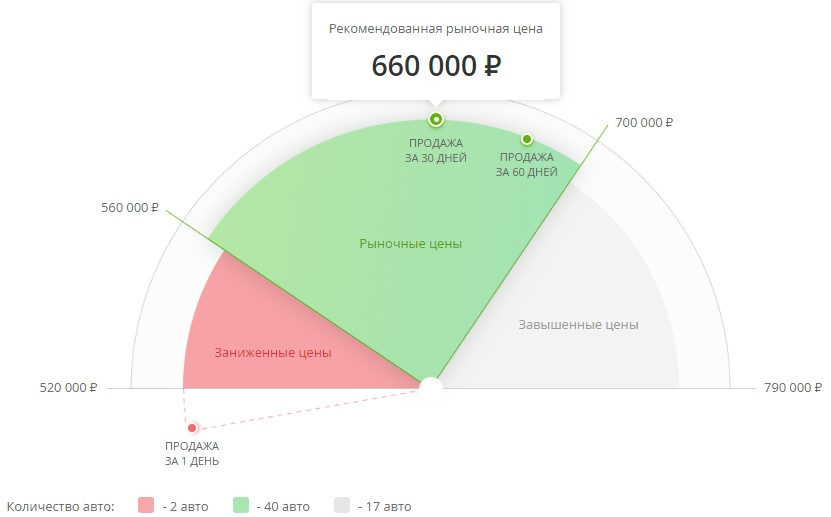
\includegraphics[width=0.98\linewidth]{images/1}
	\caption{{\footnotesize {Общие виды поврежденного ТС \тс. Фототаблица предоставлена заказчиком}}}
	\label{ris:images/1}
\end{figure}
 
Согласно сведениям, содержащимся в предоставленных материалах, \osm \, экс\-пертом-техником Яковлевым С.В. проведен осмотр поврежденного транспортного средства \tc.\,
% Осмотр проводился в сухую, ясную погоду с 14 час. 00 мин. до 14 час. 30 мин. на открытой площадке по адресу:  г. Краснодар, ул. Кореновская, 24. При осмотре присутствовали: владелец ТС \tc \, \владелец. 
Соответствие маркировочных обозначений на кузове представленного ТС записям в регистрационных документах ТС экс\-пертом-техником установлено. Видимые изменения конструкции ТС отсутствуют.  Представленный на исследование автомобиль \tc\, имеет кузов типа "\типкузова". Кузов автомобиля окрашен рефлексной %(лессирующей) 
с "металлическим" эффектом эмалью %(краской) 
синего цвета.

\renewcommand\baselinestretch{0.86}\small\normalsize 
\subsection{\underline{По  вопросу}\, \, \,	\textbf{\small{<<Установить наличие, характер и объем (степень) технических повреждений транспортного средства  \tc \,>>?}}}
\renewcommand\baselinestretch{1.2}\small\normalsize
%
% 1.\ Наличие, характер и объем технических повреждений, а так же  планируемые (предполагаемые) ремонтные воздействия для восстановления поврежденного автомобиля  исследованы в присутствии заинтересованных лиц, зафиксированы в акте осмотра № 006/06/19  от \osm% \NomerDoc \, (Приложение №1)
% ,  и фотоматериалах по принадлежности (Приложение №2). 
%
Первичное установление наличия и характера повреждений транспортного средства, в отношении которых определяются расходы на восстановительный ремонт, в соответствии с  Единой методикой определения размера расходов на восстановительный ремонт 
%в отношении поврежденного транспортного средства  
утверждены Положением Банка России от «19» сентября 2014 года № 432-П (Единой методикой), должно производится во время осмотра транспортного средства и фиксироваться актом осмотра, в который  должны включаться сведения о повреждениях транспортного средства, с обязательной  характеристикой поврежденных элементов с указанием расположения, вида и объема повреждения.   
%
В акте № 006/06/19  от \osm\, повреждений транспортного средства (ТС)  не содержатся установленные Единой методикой обязательные количественные показатели (характеристики) повреждений транспортного средства.  Отсутствие количественных характеристик повреждений в представленном акте осмотра предполагает его применение в настоящем исследовании исключительно в виде списка повреждений и перечня ремонтных воздействий, определенных экспертом-техником Яковлевым С.В. для восстановительного ремонта транспортного средства. %  не позволяет эксперту использовать указанный акт осмотра для объективного выбора необходимого и достаточного комплекса работ по восстановительному ремонту транспортного средства.
%
%На момент определения о проведении повторной судебной экспертизы, объект исследования неоднократно подвергался видоизменениям как при исследовании специалистом ООО "ЭКСПЕРТ", так и при производстве первичной судебной экспертизы экспертами ИП Куприянова Виктора Александровича. 
%
\par
Согласно данному акту осмотра № 006/06/19  от \osm \, для устранения повреждений ТС необходимо было произвести следующие ремонтные работы:
%\vspace{\baselineskip}  % вставка пустой строки
% 
\begin{longtable}{|p{1cm}|p{11cm}|p{3cm}|}
\caption[]{\footnotesize {Ремонтные воздействия по акту осмотра № 006/06/19 от \, \osm \, ИП Яковлева С.В.}} \label{tab:4}\\ 
	 \hline
		\rowcolor[HTML]{C0C0C0} 
	%	\multicolumn{1}{|c|}
	%	{\cellcolor[HTML]{C0C0C0}N/N} & Наименование запчасти (материала) & Ремонтное воздействие 
    %	
 \text{N/N} & Наименование запчасти (материала) & Ремонтное воздействие  \\ \hline \endhead
		\Rownum  & Панель задка  & Замена, окраска \\ \hline
		\rowcolor[HTML]{EFEFEF} 
		\Rownum  & Боковина задняя левая   & Замена, окраска \\ \hline
	    \Rownum  & Боковина задняя правая  & Замена, окраска  \\ \hline
		
\end{longtable}
%
\par Таким образом, размер восстановительных расходов (затрат) \тс\,  может быть произведен в объеме сведений, содержащихся в представленной Таблице \ref{tab:4}.
%\vspace{\baselineskip}  % вставка пустой строки
%
%\renewcommand\baselinestretch{0.86}\small\normalsize 
%\subsection{\underline{По  вопросу}\, 	\textbf{\small{2. <<Установить причины возникновения технических повреждений транспортного средства \tc \, и возможность их отнесения к рассматриваемому дорожно-транспортному происшествию (ДТП)>>?}}}
%\renewcommand\baselinestretch{1.2}\small\normalsize
%%
%%2.\ Причины возникновения технических повреждений и возможность их отнесения к
%%рассматриваемому ДТП исследованы при осмотре ТС. 
%Для определения причины возникновения повреждений, указанных в Акте осмотра ТС
%% №   (Приложение № 1) 
%экспертом-техником изучены документы, представленные Заказчиком и сведения о ДТП, с участием ТС \вин% \, по данным открытых источников https://гибдд.рф. 
%По предоставленным документам экспертом установлена причина ДТП, установлены обстоятельства ДТП, выявлены повреждения ТС и установлены причины их образования. Проведено исследование характера выявленных повреждений, сопоставление повреждений ТС потерпевшего с повреждениями ТС иных участников ДТП в соответствии со сведениями, зафиксированными в документах о ДТП. Проведена проверка взаимосвязанности повреждений на ТС с заявленными обстоятельствами ДТП, определен объем восстановительных работ (Приложение №1 Акт осмотра ТС). 
%Из открытых банков данных полиции следует, что автомобиль с VIN  \вин\,  как минимум дважды становился участником ДТП.
%Первый раз 29.06.2018  06:40, извещение о ДТП № 030046913, в котором автомобиль получил повреждения задней правой двери, заднего правого порога, заднего правого колеса, подушки SRS справа, Рис. \ref{ris:images/d1} и второй раз 22.05.2019 06:50, извещение о ДТП № 030034947, в котором автомобиль получил повреждения деталей передней левой и задней частей кузова, Рис. \ref{ris:images/d2}.
%
%
%\begin{figure}[H]\centering
%	\parbox[t]{0.49\textwidth}
%	{\centering
%		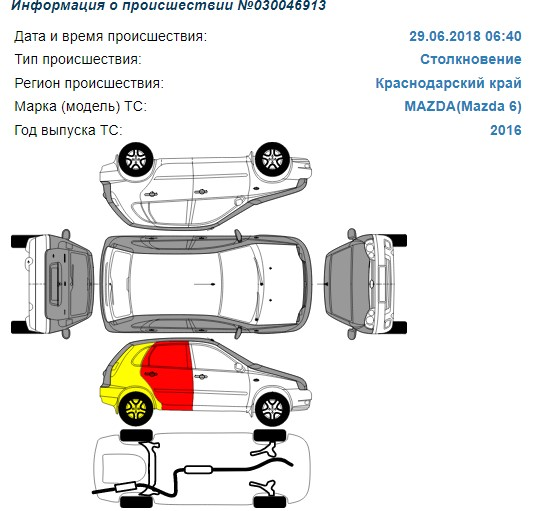
\includegraphics[width=.49\textwidth]{images/d1}
%		\caption{\footnotesize {Повреждения в ДТП 29.06.2018 }}
%		\label{ris:images/d1}}
%	\hfil \hfil%раздвигаем боксы по горизонтали 
%	\parbox[t]{0.49\textwidth}
%	{\centering
%		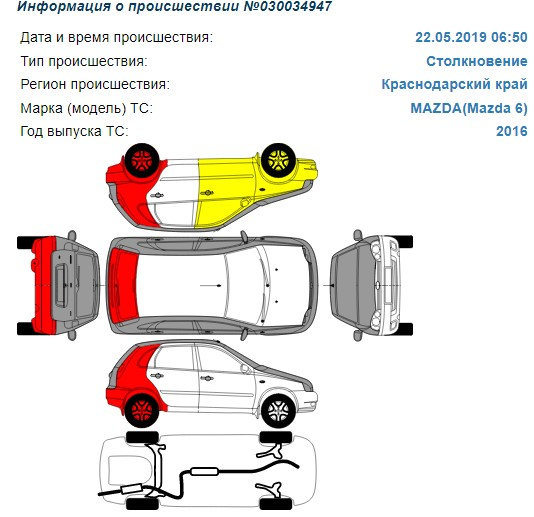
\includegraphics[width=.49\textwidth]{images/d2}
%		\caption{\footnotesize {Повреждения в ДТП 22.05.2019}}
%		\label{ris:images/d2}}
%\end{figure}
%%
%{\noindent  \footnotesize \tikz \fill [red] (1,0.5) rectangle (0.1,0.1); --{\footnotesize  Вмятины, вырывы, заломы, перекосы, разрывы и другие повреждения с изменением геометрии элементов (деталей) кузова и эксплуатационных характеристик ТС.}\\
%\tikz \fill [yellow] (1,0.5) rectangle (0.1,0.1); --  {\footnotesize Повреждения колёс (шин), элементов ходовой части, стекол, фар, указателей поворота, стоп-сигналов и других стеклянных элементов (в т.ч. зеркал), а также царапины, сколы, потертости лакокрасочного покрытия или пластиковых конструктивных деталей и другие повреждения без изменения геометрии элементов (деталей) кузова и эксплуатационных характеристик ТС.}\\[1mm]
%%%%%%%%%%%%%%%%%%%%%%%%%%%%%%%%%%%%%%%%%%%%%%%%%%%%%%%%%%%%%%%%%%%%%%%%%%%}%%%%%%%%%%%%%%%%%%%%%%%%%%%%%%%%%%%%%%%%%%%%%%%%%%
%
%\renewcommand\baselinestretch{1.2}\small\normalsize
%\begin{spacing}{1.25}Таким образом, перечень повреждений, указанный в акте осмотра № 006/06/19 от \osm \, ИП Яковлева С.В. может соответствовать повреждениям автомобиля \тс\,, полученным в результате ДТП \датадтп. 
%\end{spacing}
%\renewcommand\baselinestretch{0.86}\small\normalsize 
%\subsection{\underline{По  вопросу}\, \, \,	\textbf{\small{3. <<Установить технологию, объем восстановительного  ремонта транспортного средства \tc \,>>?}}}
%\renewcommand\baselinestretch{1.2}\small\normalsize
%%%%%%%%%%%%%%%%%%%%%%%%% Для автомобилей, старше семи лет:
%Колесное транспортное средство сроком эксплуатации более 7 лет относится к категории транспортных средств с граничным сроком эксплуатации [1], для которой возможно применение ремонтных операций при условии экономической целесообразности и  технической возможности.  
%
\renewcommand\baselinestretch{0.86}\small\normalsize 
\subsection{\underline{По  вопросу}\, \, \,	\textbf{\small{<<Установить размер затрат на восстановительный ремонт (с учётом износа) транспортного средства \tc \,>>?}}}
\renewcommand\baselinestretch{1.2}\small\normalsize
%
В соответствии с существующей экспертной методикой размер расходов на восстановительный ремонт определяется исходя из стоимости ремонтных работ (работ по восстановлению, в том числе окраске, контролю, диагностике и регулировке, сопутствующих работ), стоимости используемых в процессе восстановления транспортного средства деталей (узлов, агрегатов) и материалов взамен поврежденных. 
%                                         
%В соответствии с принятой экспертной методикой [1], стоимость восстановительного ремонта АМТС  $ C_p $ определяется по формуле:
%%
%\begin{equation}\label{eq:r}
%C_\text{вp} =C_p + C_\text{м} + C_\text{зч}\cdot\left( 1-\frac{\text{И}}{100}\right)  \,\,\,\, \text{где:}
%\end{equation}
%%
%%
%\begin{itemize}
%%	
%\item[ ]$C_\text {р} $ --  стоимость ремонтных работ по восстановлению КТС, руб.;
%\item[ ]$ C_\text{м} $ --  стоимость необходимых ремонтных материалов, руб.;
%\item[ ]$ C_\text{зч} $ --  стоимость новых запасных частей, руб;
%\item[ ] $ \text{И} $ -- коэффициент износа составной части, подлежащей замене, \%.
%\end{itemize}
%%
%%
%Коэффициент износа составных частей (И) КТС (кроме автобусов и грузовых автомобилей) при определении стоимости восстановительного ремонта расчитывается по формуле:
%
%\begin{equation}\label{eqsnos}
%\text{И} =\text{И1}\cdot\text{П}+\text{И2}\cdot \text{Д}, \%  \,\,\,\, \text{где:}
%\end{equation}
%
%\begin{itemize}
%	\item [] $ \text{И1} $ --усредненный показатель износа на 1000 км пробега, \%; 
%	\item [] $ \text{П} $ -- общий пробег (фактический или расчетный) за срок эксплуатации КТС, тыс.км;
%	\item [] $ \text{И2} $ -- усредненный показатель старения за 1 год эксплуатации, \%;
%	\item [] $ \text{Д} $ -- срок эксплуатации КТС (от даты изготовления КТС до момента, на который определяется износ), лет. 
%\end{itemize}
%
%Для исследуемого автомобиля \тс, согласно справочным таблицам [1]:
%\begin{equation}\label{eqsnosr}
%\text{И} =\text{И1}\cdot\text{П}+\text{И2}\cdot \text{Д} = 0.23\cdot 214  + 0.85\cdot 9 = 49 \, \%
%\end{equation}
%%%%%%%%%%%%%%%%%%%%%%%%%%%%%%%%%%%%%%%%%%%%%%%%%%%%%%%%%%%%%%%%%%%%%%%%%%%%%%%%%%%%%%%%%%%%%%%%%%%%%%%%%%%%%%%%
Стоимость восстановительных работ $ C_{\text{вр}} $ определяется на основании норм трудоёмкостей $ T_i $, \, предусмотренных заводом-изготовителем, и стоимостных параметров $ C_{i\text{нч}} $ (стоимости нормо-часа) работ по техническому обслуживанию и ремонту АМТС.  Расчет размера расходов (в рублях) на восстановительный ремонт производится по формуле:
\begin{equation}\label{eq:cr}
C_{\text{вр}}  =\sum{C_{ip}}= \sum\left({T_{ij}}\cdot {C_{i\text{нч}}}\right) + \sum{C_{ip^{\text{\,\,\,руб}}}} , \,\,\,\text{где:} 
\end{equation}
%\vspace{2mm}
\begin{itemize}
	\item[ ]$ C_{ip} $ -- стоимость работ i-го вида: $C_\text {зам} $, $ C_\text{восст} $, $ C_\text{рег} $, $C_\text{контр} $, $ C_\text{антикор} $, $ C_\text{зч} $, $ C_\text{ом} $,$ C_\text{соп} $, $ C_\text{вм} $, руб;
	\item[ ]$ T_{ij} $ -- трудоёмкость j-й операции(комплекса) по i-му виду работ, руб;
	\item[ ]$ C_{i\text{нч}} $ -- стоимость нормо-часа по i-му виду работ, руб;
	\item[ ]$ C_{ip^\text{\,\,руб}} $ -- стоимость работ $ C_{ip} $, принятая непосредственно в денежном выражении, руб.
\end{itemize}
%
\par При определении стоимости восстановительного ремонта АМТС с учётом износа под износом следует понимать количественную меру физического старения АМТС и его элементов, достигнутого в результате эксплуатации, т.е. эксплуатационный износ.
%
Расчёт износа производится в  соответствии с Положением Банка России от «19» сентября 2014 года № 432-П «О единой методике определения размера расходов на восстановительный ремонт в отношении повреждённого транспортного средства» [2].
Износ комплектующих изделий (деталей, узлов, агрегатов) рассчитывается по следующей формуле:
%
\begin{equation}\label{eq:I}
\text{И}_{\text{ки}} 
= 100\cdot\left( 1-e^ {-\left( \Delta_{T} \cdot T_{\text{КИ}} + \Delta_{L} \cdot L_{\text{КИ}} \right)}\right), \,\,\,\,\text{где:}   
\end{equation}
%
\begin{itemize}
	\item[ ]$ \text{И}_{\text{ки}} $ -- износ комплектующего изделия (детали, узла, агрегата) (процентов); 
	\item[ ]$ e $ -- основание натуральных логарифмов (e =  2,72);
	\item[ ]$ \Delta_{T}$ --  срок эксплуатации комплектующего изделия (детали, узла, агрегата) (лет);
	\item[ ]$ T_{\text{КИ}} $ -- стоимость работ $ C_{ip} $, принятая непосредственно в денежном выражении, руб
	\item[ ]$ \Delta_{L} $ --коэффициент, учитывающий влияние на износ комплектующего (детали, узла, агрегата) величины пробега транспортного средства с этим комплектующим изделием;
	\item[ ]$ L_{\text{КИ}} $ --пробег транспортного средства на дату дорожно-транспортного происшествия (тысяч километров).  
		\end{itemize}
\vspace{5mm}
\par Значения коэффициентов $ \Delta_{T}$  и $ \Delta_{L} $  для различных категорий и марок транспортных средств приведены в п.5. сп. лит~[2]. При этом, на комплектующие изделия (детали, узлы, агрегаты), которые находятся в заведомо худшем состоянии, чем общее состояние транспортного средства в целом, и его основные части, вследствие влияния факторов, не учтённых при расчете износа (например, проведение ремонта с нарушением технологии, не устранение значительных повреждений лакокрасочного покрытия), может быть начислен дополнительный индивидуальный износ. 
Износ шины транспортного средства рассчитывается по следующей формуле:
\begin{equation}\label{eq:sh}
\text{И}_{\text{ш}} = \frac{\text{Н}_{\text{н}}-\text{Н}_{\text{ф}}}{\text{Н}_{\text{н}}-\text{Н}_{\text{доп}}} \cdot{100}\%  \,\,\,\,\text{где:} 
\end{equation}
%
\begin{itemize}
	\item[ ] $ \text{И}_{\text{ш}} $ -- износ шины, \%;
	\item[ ] $ \text{Н}_{\text{н}} $ -- высота рисунка протектора новой шины, мм;
	\item[ ] $\text{Н}_{\text{ф}} $ -- фактическая высота рисунка протектора шины, мм;
	\item[ ] $ \text{Н}_{\text{доп}} $ --минимально допустимая высота рисунка протектора шины в соответствии с требованиями законодательства Российской Федерации, мм.
\end{itemize}
%
\vspace{5mm}
\renewcommand\baselinestretch{1}\small\normalsize
%
%Износ шины дополнительно увеличивается для шин с возрастом от 3 до 5 лет - на 15 процентов, свыше 5 лет - на 25 процентов.
%%%%%%%%%%%%%%%%%%%%%%%%%%%%%%%%%%%%%%%%%%%%%%%%%%%%%%%%%%%%%%%%%%%%%%%%%%%%%%%%%%%5
%В результате исследования   экспертом-техником установлено, что для устранения повреждений \тс \, необходимо  выполнить следующие  работы:
%\begin{center}
%	\begin{tabulary}{\textwidth}{LCL}
%\hline 
%\textbf{Наименование детали}      &   & \textbf{Ремонтное воздействие}\\
%\hline Турбина левая              &   &    Заменить\\
%Блок ДВС                          &   &    Отремонтировать гильзованием, заменой колец и прокладок \\
%	\end{tabulary}  
%\end{center}
%%%%%%%%%%%%%%%%%%%%%%%%%%%%%%%%%%%%%%%%%%%%%%%%%%%%%%%%%%%%%%%%%%%%%%%%%   CSV    %%%%%%%%%%%%%
%\csvautobooklongtable[separator=comma]{test.csv} % semicolon- ;  comma- , pipe- | tab- 	
%%%%%%%%%%%%%%%%%%%%%%%%%%%%%%%%%%%%%%%%%%%%%%%%%%%
%%%%%%%%%%%%%%%%%%%%%%%%%%%%%%%%%%%%%%%%%%%%%%%%%%%%%%%%%%%%%%%%%%%%%%%%%%%%%%%%%
%
%%%%%%%%%%%%%%%%%%%%%%%%%%%%%%%%%%%%%%%%%%%%%%%%%%%%%%%%%%%%%%%%%%%%%%%%%%%%%%%%%
%
%%%%%%%%%%%%%%%%%%%%%%%%%%%%%%%%%%%%%%%%%%%%%%%%%%%%%%%%%%%%%%%%%%%%%%%%%%%%%%%%5
\renewcommand\baselinestretch{1.2}\small\normalsize
%%
%\textbf{Произвести  необходимые для выполнения  ремонта разборочно-сборочные, подготовительные и вспомогательные работы в соответствии с требованиями завода–изготовителя транспортного средства.}\\
%%
Расчет стоимости восстановительных расходов выполнен в программе \auda\, в модуле ОСАГО ПРО. Процент износа ТС \тс\, так же произведен в указанной программе, на момент  исследуемого страхового события составлял 22.96\%. \par Ниже представлены результаты расчета, полная калькуляция стоимости ремонта включена в раздел <<Приложение>> настоящего заключения.
%%\smallskip
\begin{figure}[H]
	\centering
	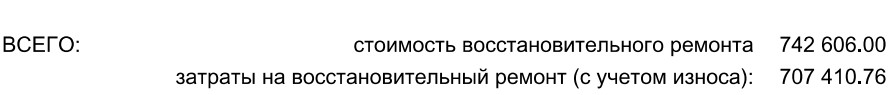
\includegraphics[width=0.8\linewidth]{images/Screenshot_2}
%%	\caption{}
%%	\label{fig:screenshot001}
\end{figure}
%\begin{figure}[H]
%	\centering
%	\includegraphics[width=0.9\linewidth]{images/screenshot002}
%%%	\caption{}
%	\label{aud}
%\end{figure}
\medskip
\renewcommand\baselinestretch{1.2}\small\normalsize
%%%%%%%%%%%%%%%%  Если не ОСАГО
%Стоимость коммерческого нормо-часа работ применена  с учетом условий регионального рынка услуг и сложившихся средних расценок по видам работ, типу ТС, а также по маркам и моделям ТС  и   составляет  1300 р/ч для данного транспортного средства. \\
%Трудоёмкость работ по разборке/сборке/замене  соответствует трудоемкости работ, рекомендованной заводом изготовителем ТС. 
%Расчет стоимости ремонта, согласно положениям [1] производится с учетом  применения оригинальных запасных частей, которые поставляются изготовителем КТС авторизованным ремонтным организациям. Техническое состояние запасных частей учитывается коэффициентом износа, что в совокупности с установкой оригинальных запасных частей в максимальной степени отвечает понятию «восстановительный ремонт», то есть восстановления состояния КТС, при котором используются установленные изготовителем составные части, но с использованным частично ресурсом. 
%
%%%%%%%%%%%%%%%%%% Если ОСАГО
Стоимость одного нормо-часа работ определена в соответствии с пунктом 3.8.1 Единой методики [2] путем применения электронных баз данных стоимостной информации.
Трудоемкость работ по разборке/сборке/замене  соответствует трудоемкостям работ, рекомендованным заводом изготовителем ТС. Трудоемкости окрасочных работ приняты в соответствии с технологией  AZT (http://www.schwacke.ru/down/azt \_reparaturlackierung\_ru.pdf). Расчет размера расходов на материалы произведен  согласно пункту 3.7.2 Приложения к Единой методике [2]. 
Стоимость запасных частей определена в соответствии с пунктом 3.6.3 Единой методики путем применения электронных баз данных стоимостной информации.
% (по утвержденному справочнику: http://prices.autoins.ru/priceAutoParts/repair\_parts.html.
%
\par Таким образом, в результате проведенных расчетов (см. Приложение, калькуляция \NomerDoc) определена стоимость восстановительного ремонта транспортного средства  \тс, которая составляет 1\,085\,696 (Один миллион восемьдесят пять тысяч шестьсот девяносто шесть) рублей без учета износа,
стоимость восстановительных расходов, с учетом уменьшения стоимости запасных частей вследствие их износа,  составляет 871\,841 (Восемьсот семьдесят одна тысяча восемьсот сорок один) рубль, что с учетом округления составляет 871\,800 (Восемьсот семьдесят одна тысяча восемьсот) рублей.
\nopagebreak
\include{rinok}
\paragraph*{Расчет стоимости годных остатков.}
 Стоимость годных остатков с учетом затрат на их демонтаж, дефектовку, хранение и продажу определяется по формуле:
 \begin{equation}\label{go}
C_{\text{ГО}}= C_{\text{Р}} \cdot K_{\text{В}}\cdot K_{\text{З}}\cdot K_{\text{ОП}} \cdot  \sum\limits_{i-1}^{n}\frac{C_i}{100}, \, \, \text{руб} 
\end{equation}
\noindent где: \,$ C_{\text{Р}} $ -- стоимость ТС в неповрежденном виде на момент происшествия;\\
$ K_{\text{З}} $-- коэффициент, учитывающий затраты на дефектовку, разборку, хранение, продажу;\\
$ K_{\text{В}} $ -- коэффициент, учитывающий срок эксплуатации АМТС на момент повреждения и спрос на его неповрежденные детали;\\
$ K_{\text{ОП}} $ -- коэффициент, учитывающий объем (степень) механических повреждений автомобиля;\\
$ C_i $ процентное соотношение (вес) стоимости неповрежденных элементов к стоимости автомобиля;\\
$ n  $- количество неповрежденных элементов (агрегатов, узлов).\\

Расчет процентного соотношения (веса) стоимости неповрежденных элементов к стоимости ТС   \,\,
     % \begin{equation}\label{bb}
   $  \left( \sum\limits_{i-1}^{n}\frac{C_i}{100} \right)  $  
%   \end{equation}  
включает только установленные неповрежденные детали, узлы и агрегаты. Компоненты ТС, имеющие повреждения  вероятностного характера, и требующие диагностических работ для установления годности в расчете не учитываются. 
 
  \begin{longtable}{|p{9cm}|p{4cm}|p{2cm}|}
 	\caption[]{\footnotesize {Таблица расчета $ C_i $ }}
 	 \label{tab:7}\\
 	 \hline
 	 		Наименование агрегата, узла, детали & \%-ное соотношение (вес)  & Годные, \% \\
 	 		\hline \endhead
 		Кузовные детали, экстерьер, интерьер, в т.ч.: & 50 (45 \textless{}1\textgreater{}) & 0 \\
 		Передняя часть: & 14 &  \\
 		Капот & 1.9 & 1,9 \\
 		Крыло переднее (за 1 шт.) & 0.8 & 0,8 \\
 		Бампер передний (в сборе с усилителем, накладками и молдингами, спойлером) & 1.9 & 1,9 \\
 		Решетка (облицовка) радиатора & 0.8 & 0,8 \\
 		Лонжерон передний (за 1 шт.) & 0.8 & 0,8 \\
 		Брызговик крыла (за 1 шт.) & 1.4 & 1,4 \\
 		Стекло ветрового окна & 1.7 & 1,7 \\
 		Рамка радиатора & 1.4 & 1,4 \\
 		Щиток передка & 0.3 & 0,3 \\
 		Задняя часть: & 12 (14 \textless{}1\textgreater{}) & 0 \\
 		Бампер задний & 1.6 & 0 \\
 		Крыло заднее (боковина \textless{}1\textgreater{}) в сборе с арками (за 1 шт.) & 2.1 (3.1 \textless{}1\textgreater{}) & 0 \\
 		Стекло окна задка & 1.9 & 0 \\
 		Панель задка & 0.8 & 0 \\
 		Пол багажника & 0.8 & 0 \\
 		Облицовки багажника & 1.1 & 0 \\
 		Крышка багажника (дверь задка) & 1.6 & 0 \\
 		Средняя часть: & 24 (17 \textless{}1\textgreater{}) & 0 \\
 		Передняя стойка боковины (за 1 шт.) & 1.4 & 2,8 \\
 		Средняя стойка боковины с порогом и частью пола (за 1 шт.) & 1.4 (0 \textless{}1\textgreater{}) & 2,8 \\
 		Облицовки стоек боковины, порогов, уплотнители, центральная консоль, противосолнечные козырьки, плафоны освещения, коврики пола, зеркало заднего вида & 2.5 (2.1 \textless{}1\textgreater{}) & 2,5 \\
 		Двери в сборе с арматурой (за 1 шт.), & 1.9 & 5,7 \\
 		в т.ч. арматура дверей (за 1    дверной комплект) & 0.5 & 0 \\
 		Сиденья (все) & 1.1 & 1,1 \\
 		Панель крыши в сб. с обивкой, поперечинами и верх. частями стоек, & 3.5 & 2,7 \\
 		в т.ч. обивка панели крыши & 0.8 & 0 \\
 		Панель приборов в сборе с щитком приборов, решетками, вещевым ящиком, карманами и т.д. & 2.5 & 2,5 \\
 		Ремень безопасности передний (за 1 шт.) & 0.3 & 0,6 \\
 		Подушка безопасности пассажирская & 0.6 & 0,6 \\
 		Двигатель, навесное, охлаждение, впускная и выпускная система & 11 (13 \textless{}2\textgreater{}) & 13 \\
 		Двигатель в сборе без навесного оборудования & 4.9 & 0 \\
 		в т.ч. клапанная крышка & 0.5 & 0 \\
 		в т.ч. масляный поддон & 0.5 & 0 \\
 		в т.ч. блок цилиндров & 2.2 & 0 \\
 		Дроссельный узел в сборе с заслонкой, клапаном и датчиком & 1.4 & 0 \\
 		Генератор & 0.8 & 0 \\
 		Коллектор впускной & 0.5 & 0 \\
 		Коллектор выпускной & 0.5 & 0 \\
 		Радиатор охлаждения в сборе с кожухами, вентилятором & 0.8 & 0 \\
 		Стартер & 0.5 & 0 \\
 		Короб воздушного фильтра с патрубками & 0.5 & 0 \\
 		Выпускной тракт в сборе & 0.8 & 0 \\
 		Турбокомпрессор (турбонагнетатель) & 1.4 \textless{}2\textgreater{} & 0 \\
 		Интеркулер & 0.6 \textless{}2\textgreater{} & 0 \\
 		Топливная система & 2.5 & 2,5 \\
 		Бак топливный & 0.7 & 0 \\
 		Система подачи топлива & 1.8 & 0 \\
 		Трансмиссия & 4.5 & 4,5 \\
 		Усредненный показатель с учетом всех возможных вариантов трансмиссии & 4.5 & 0 \\
 		Подвеска & 10 & 4 \\
 		Подвеска передняя в сборе с поперечиной & 5.5 (4.5 \textless{}4\textgreater{}) & 0 \\
 		Подвеска задняя в сборе с поперечиной & 4.5 (5.5 \textless{}4\textgreater{}) & 4,5 \\
 		Подвеска в сборе для полноприводных АМТС & 10 (5 \textless{}4\textgreater + 5 \textless{}4\textgreater{}) & 0 \\
 		Рулевое управление & 3 & 3 \\
 		Рулевая колонка в сборе с валом & 0.5 & 0 \\
 		Насос ГУР & 0.8 & 0 \\
 		Рулевой механизм & 1.2 & 0 \\
 		Рулевое колесо в сборе с подушкой безопасности & 0.5 & 0 \\
 		в т.ч.: подушка безопасности  водительская & 0.3 & 0 \\
 		Тормозная система & 3.5 & 3,5 \\
 		Главный тормозной цилиндр & 0.5 & 0 \\
 		Тормозной механизм колеса (за каждый колесный узел) & 0.5 & 0 \\
 		Ручной (ножной) тормоз & 0.3 & 0 \\
 		Блок управления АБС & 0.7 & 0 \\
 		Электрооборудование & 12.5 & 0 \\
 		Провода свечные с катушками (комплект) & 0.5 & 0,5 \\
 		Монтажный блок & 0.5 & 0,5 \\
 		Блок управления двигателем & 1 & 1 \\
 		Фонари задние (за 1 шт.) & 0.5 & 1 \\
 		Зеркала заднего вида боковые (за 1 шт.) & 0.8 & 1,6 \\
 		Блок отопителя салона в сборе (корпус, двигатель, радиаторы) & 2.1 & 2,1 \\
 		Насос кондиционера & 0.5 & 0,5 \\
 		Конденсатор в сборе с осушителем, кожухом, вентилятором, трубками & 0.6 & 0,6 \\
 		Фары (за 1 шт.) & 1.1 & 1,1 \\
 		Жгут проводов ДВС & 0.9 & 0,9 \\
 		Жгут проводов панели приборов & 0.8 & 0,8 \\
 		Остальные жгуты проводов (все) & 0.3 & 0,3 \\
 		Фара противотуманная (за 1 шт.) & 0.8 & 1,6 \\ 
 		Прочее & 3/8 \textless{}1\textgreater{}/1 \textless{}2\textgreater /6 \textless{}3\textgreater{} & 4 \\
 		\hline
 		\textbf{ИТОГО,} \%: &  & \textbf{83,8}  \\
 		\hline	
 	\end{longtable}
 
\noindent  \begin{table}[H]
  	 \label{tab:KB}
	\caption{\footnotesize {Значения коэффициента Кв, учитывающего срок эксплуатации ТС}}
		 \begin{tabular}{|p{47mm} |p{53mm}| p{50mm}|}
	\hline
 		Срок эксплуатации автомобиля, лет & Значение Кв легковых автомобилей, малотоннажных грузовых на базе легковых и мототехники & Значение Кв грузовых автомобилей \\ \hline
 		0 - 5 (включительно)              & 0.80                                                                                    & 0.80                             \\ \hline
 		6 - 10 (включительно)             & 0.65                                                                                    & 0.60                             \\ \hline
 		11 - 15 (включительно)            & 0.55                                                                                    & 0.50                             \\ \hline
 		16 - 20 (включительно)            & 0.40                                                                                    & 0.35                             \\ \hline
 		Более 20 лет                      & 0.35                                                                                    & 0.30                            \\ \hline
 	\end{tabular}
\end{table}


\noindent \begin{table}[H]
	\label{tab:KO}
	\caption{\footnotesize {Значение коэффициента $ K_{\text{оп}} $ , учитывающего объем (степень) механических повреждений автомобиля}} 
	\centering
\begin{tabular}{|p{47mm}| p{53mm}| p{50mm}|}
	\hline
	Объем механических повреждений & Соотношение стоимости неповрежденных элементов к стоимости автомобиля, Ci, \% & Значение коэффициента, учитывающего объем механических повреждений \\ \hline
	Незначительный                 & 80 - 100                                                                      & 0.9 - 1                                                            \\
	& 60 - 80                                                                       & 0.8 - 0.9                                                          \\
	Средний                        & 40 - 60                                                                       & 0.7 - 0.8                                                          \\
	& 20 - 40                                                                       & 0.6 - 0.7                                                          \\
	Значительный                   & 0 - 20                                                                        & 0.5 - 0.6                                                          \\ \hline
\end{tabular}
\end{table}

 \par
 
% \begin{equation}\label{k}
% C_{\text{ГО}}= C_{\text{Р}} \cdot K_{\text{В}}\cdot K_{\text{З}}\cdot K_{\text{ОП}} \cdot  \sum\limits_{i-1}^{n}\frac{C_i}{100} 
% \end{equation}
 
 Для исследуемого транспортного средства применимы следующие значения коэффициентов:\par
 $ K_{\text{В}} =0.8  $; 
 $ K_{\text{З}} =0.7 $; 
 $ K_{\text{ОП}} =0.8 $; $ \sum\limits_{i-1}^{n}\frac{C_i}{100} = 0.838 $ \par тогда:
 \par
$  C_{\text{ГО}} =  C_{\text{ГО}}= C_{\text{Р}} \cdot K_{\text{В}}\cdot K_{\text{З}}\cdot K_{\text{ОП}} \cdot  \sum\limits_{i-1}^{n}\frac{C_i}{100} =980000*0.8*0.7*0.8*0.838 = 367915 $ руб., или с учетом округления 370 000 (Триста семьдесят тысяч) рублей.
\par Таким образом, стоимость годных остатков ТС \тс \, \, составляет 370 000 (Триста семьдесят тысяч) рублей.


%
\section{Выводы}
%
%
\begin{enumerate}
 \item  Наличие, характер и объем (степень) технических повреждений, причиненных ТС, определены при осмотре и зафиксированы в Акте осмотра \NomerDoc.
 % \, и фототаблице повреждений, являющимися неотъемлемой частью настоящего экспертного заключения.
 \\[-2mm]

%\item  Направление, расположение и характер повреждений определены путем сопоставления полученных повреждений, изучения административных материалов по рассматриваемому событию, и  являются  следствиями рассматриваемого ДТП (события).\\[-2mm]

\item  Технология и объем необходимых ремонтных воздействий зафиксированы в калькуляции \NomerDoc \, по определению стоимости восстановительного ремонта транспортного средства \тс. Расчетная стоимость восстановительного ремонта составляет 1\,085\,696 (Один миллион восемьдесят пять тысяч шестьсот девяносто шесть) рублей.
\\[-2mm]
\item  Размер затрат на проведение восстановительного ремонта с учётом износа (восстановительные расходы) транспортного средства \тс \, составляет 871\,800 (Восемьсот семьдесят одна тысяча восемьсот) рублей  рублей.\\[-2mm]   
\item Рыночная стоимость транспортного средства ТС \тс\, на момент повреждения составляла  980000 (Девятьсот восемьдесят тысяч рублей). \\[-2mm]
\item Стоимость годных остатков ТС \тс \, \, составляет 370 000 (Триста семьдесят тысяч) рублей.
\end{enumerate}
\vspace{15mm}
\relax
Приложение к заключению:\\
\textit{
	Приложение № 1. Расшифровка модельных опций ТС \тс \\
	Приложение № 2. Калькуляция стоимости восстановительных расходов ТС \тс\\
%	Приложение № 3. Цифровые копии регистрационных документов ТС\\
%	Приложение № 4. Цифровая копия постановление по делу об административном правонарушении дорожно-транспортном происшествии\\
	Приложение № 3. Правоустанавливающие документы\\
	   }

\vspace{20mm}
%\newlength{\ML}
{Эксперт-техник}\hfill           {Мраморнов А.В.}


%\includepdf[pages=-]{myfile.pdf}

%\includepdf[pages=-]{calc.pdf}